\section{Burst Ranges}

The following diagrams show the space each character can cover within 18 frames.

18 Frames is considered the lower bound of human reaction time in smash ultimate. 20-21 frames is more realistic for most players. See section \ref{sec:reaction-times} for more information on human reaction times.

\begin{multicols}{2}

\subsection{Mario}
\subsection{Donkey Kong}
\subsection{Link}
\subsection{Samus \& Dark Samus}
\subsection{Yoshi}
\subsection{Kirby}
\subsection{Fox}
\begin{figure}[H]
    \centering
    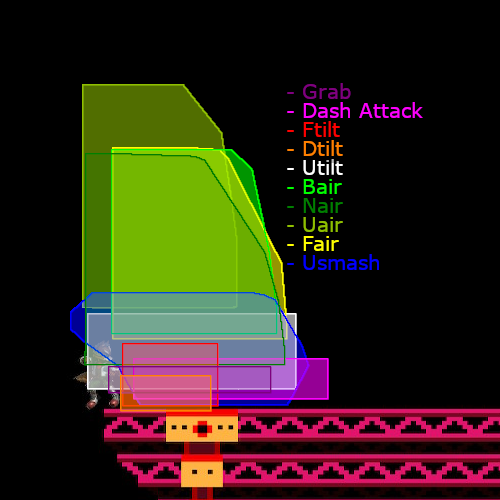
\includegraphics[width=.45\textwidth]{images/burst-ranges/fox}
    \caption{Fox's 18-frame burst range\cite{ref:burst-range:fox}}
\end{figure}

\subsection{Pikachu}
\begin{figure}[H]
    \centering
    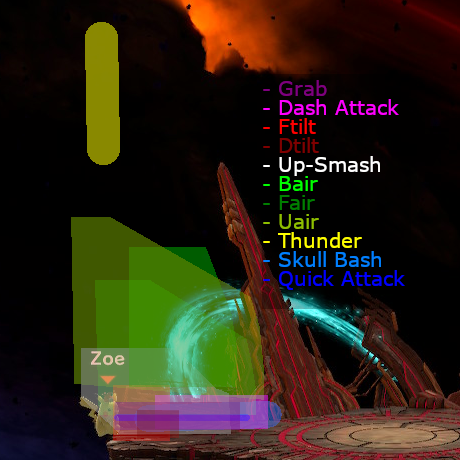
\includegraphics[width=.45\textwidth]{images/burst-ranges/pika}
    \caption{Pikachu's 18-frame burst range\cite{ref:burst-range:pika}}
\end{figure}

\subsection{Luigi}
\subsection{Ness}
\subsection{Captain Falcon}
\begin{figure}[H]
    \centering
    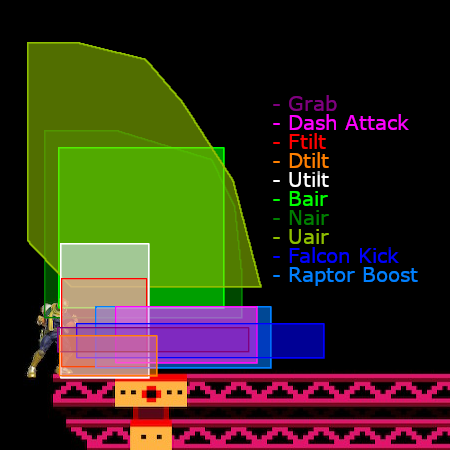
\includegraphics[width=.45\textwidth]{images/burst-ranges/falcon}
    \caption{Captain Falcon's 18-frame burst range\cite{ref:burst-range:falcon}}
\end{figure}

\subsection{Jigglypuff}
\subsection{Peach \& Daisy}
\subsection{Bowser}
\subsection{Ice Climbers}
\subsection{Sheik}
\begin{figure}[H]
    \centering
    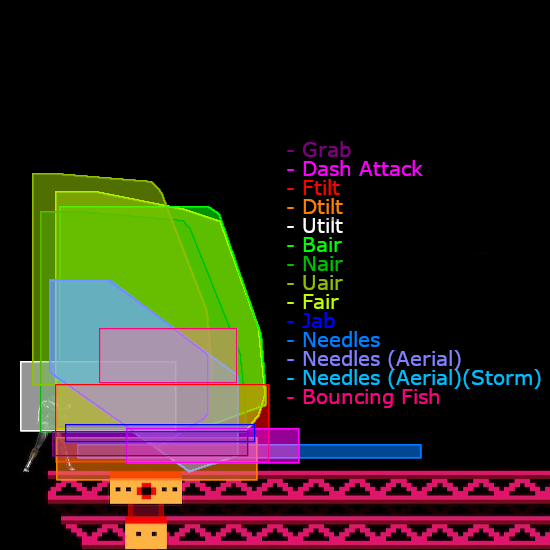
\includegraphics[width=.45\textwidth]{images/burst-ranges/sheik}
    \caption{Sheik's 18-frame burst range\cite{ref:burst-range:sheik}}
\end{figure}

\subsection{Zelda}
\subsection{Dr. Mario}
\subsection{Pichu}
\subsection{Falco}
\subsection{Marth \& Lucina}
\subsection{Young Link}
\subsection{Ganon}
\subsection{Mewtwo}
\subsection{Roy \& Chrom}
\subsection{Mr. Game and Watch}
\subsection{Meta Knight}
\subsection{Pit \& Dark Pit}
\subsection{Zero Suite Samus}

\subsection{Wario}
\begin{figure}[H]
    \centering
    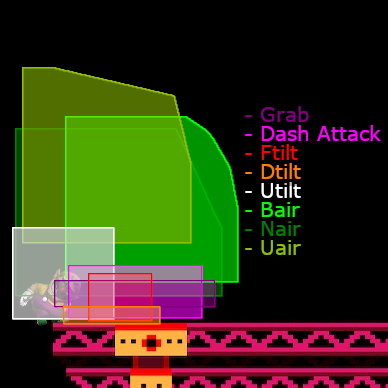
\includegraphics[width=.45\textwidth]{images/burst-ranges/wario}
    \caption{Wario's 18-frame burst range\cite{ref:burst-range:wario}}
\end{figure}
\subsection{Snake}
\subsection{Ike}
\subsection{Pok\'emon Trainer}
\subsection{Diddy}
\subsection{Lucas}
\subsection{Sonic}
\subsection{King Dedede}
\subsection{Olimar}
\subsection{Lucario}
\subsection{Rob}
\subsection{Toon Link}
\subsection{Wolf}
\subsection{Villager}
\subsection{Megaman}
\subsection{Wii Fit Trainer}
\subsection{Rosalina \& Luma}
\subsection{Little Mac}
\subsection{Greninja}
\subsection{Mii Brawler}
\subsection{Mii Swordfighter}
\subsection{Mii Gunner}
\subsection{Palutena}
\subsection{Pac-Man}
\subsection{Robin}
\subsection{Shulk}
\subsection{Bowser Jr.}
\subsection{Duck Hunt}
\subsection{Ryu \& Ken}
\subsection{Cloud}
\subsection{Corrin}
\begin{figure}[H]
    \centering
    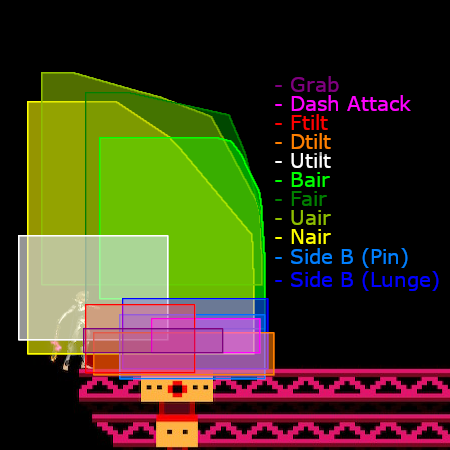
\includegraphics[width=.45\textwidth]{images/burst-ranges/corrin}
    \caption{Corrin's 18-frame burst range\cite{ref:burst-range:corrin}}
\end{figure}

\subsection{Bayonetta}
\subsection{Inkling}
\subsection{Ridley}
\subsection{Simon \& Richter}
\subsection{King K. Rool}
\subsection{Isabelle}
\subsection{Incineroar}
\subsection{Piranha Plant}
\subsection{Joker}
\subsection{Hero}
\subsection{Banjo \& Kazooie}
\subsection{Terry}
\subsection{Byleth}
\subsection{Min Min}
\subsection{Steve}
\subsection{Sephiroth}
\subsection{Pyra/Mythra}
\subsection{Kazuya}

\end{multicols}
